% Provenance (never printed): see sources/outline_sources.md (Year 3:
% planetary atmospheres, escape, the runaway greenhouse, Mars, Titan,
% habitability).
% Brief: sources/book5/BRIEFS.md, ch. 27. Curves from figdata/bachelor-3/
% jeans_escape.py (escape parameter and escaping fraction at the exobases
% of Venus, the Earth, Mars and Titan), runaway_greenhouse.py (an
% illustrative grey model of a moist atmosphere: OLR against surface
% temperature) and habitability.py (the habitable-zone fits of Kopparapu et
% al. 2013; the phase boundaries of water and methane with the surface
% states of four bodies). Exercise and problem values in the Book 5 scratch
% calculator calc/ch27.py. Kepos and its star are invented.
\chapter{行星大气与宜居性}\label{ch:b3:planetary-atmospheres}

金星与地球堪称近似孪生：大小几乎相同，平均
密度相近，轨道相邻。然而金星保有 \qty{92}{bar} 的二氧化碳，
其表面温度为 \qty{737}{K}，而水少得可怜，若将其
平铺于表面，只能形成约一厘米深的水层。先驱者金星探测器的
质谱仪在穿越云层下降时，
测得这些水中氘与氢的比值为 \num{0.016}，
是地球海洋中该比值的一百倍。较轻的氢比较重的氘更容易逃逸
到太空中；一个大储库在失去大部分氢之后，所剩部分
富含氘。这一比值是
金星曾经拥有又已失去的水的痕迹。本章探讨一颗行星如何
留住其大气与水，又如何失去它们。
% ledger: planet:Venus.diameter, planet:Earth.diameter, planet:Venus.density, planet:Earth.density, nasa:venus-atm, arney18:venus-water, donahue82:dh, kc98:standards

\begin{recall}
标高、气压公式、麦克斯韦–玻尔兹曼
分布、逃逸速度、平均自由程和温室
效应都见于物理教材。恒星的宜居带见于
中学教材。平衡温度与邦德反照率见于
本科一年级分册的比较行星学一章；光学
厚度见于望远镜与测光一章；气温递减率见于
大气与海洋结构一章；向外
长波辐射（OLR）与发射温度见于
辐射与热量输送一章。湿绝热线见于本科二年级分册
的大气热力学一章；雪线见于
行星形成一章；长期碳循环与
硅酸盐风化恒温器见于地质
时间尺度上的气候一章。\omterm{prop:b3:stable-isotopes:rayleigh-distillation}{瑞利蒸馏}见于本册
稳定同位素一章。
\end{recall}

\section{大气的结构}\label{sec:b3:planetary-atmospheres:structure}

设分子质量为 $m$、温度为 $T$ 的等温大气，
压强随高度按 $p = p_0\,e^{-z/H}$ 减小，标高 $H = kT/mg$。
在地球表面，$H$ 约为 \qty{8}{km}；在
土卫六表面，重力弱而气温低，标高约为 \qty{20}{km}。

不过，温度并不均匀。到达地面的阳光
使地面升温；上方空气能吸收和发射红外辐射，
从下方加热。若仅有辐射，低层大气的温度
变化会过于陡峭而发生翻转。

\begin{definition}[辐射–对流平衡]\label{def:b3:planetary-atmospheres:rce}
若某一大气柱处于\emph{辐射–对流
平衡}\index{辐射–对流平衡}时，在每一高度上
辐射净通量保持平衡，但在下方一层
中对流将热量向上输送，并使温度梯度
保持在绝热值。对流的下层称为对流层，
辐射平衡的上层称为平流层；对流层顶
即两者相接的高度。
\end{definition}

能够据此讨论的最简单大气为\emph{灰大气}：
它对太阳光透明，对所有红外波长的吸收一致，
光学厚度 $\tau$ 自顶向下计算。

\begin{proposition}[灰大气辐射平衡]\label{prop:b3:planetary-atmospheres:grey}
在向空间发射通量为 $F$ 的辐射平衡灰大气中，
光学厚度为 $\tau$ 处的温度满足
\[
\sigma T^4(\tau) = \frac F2\,(1 + D\tau),
\]
其中 $D \approx 1.66$ 考虑了辐射的斜程路径。
大气顶部的温度为\emph{表层温度}，
即 $T_\mathrm{skin} = 2^{-1/4}\,T_e$，其中 $T_e = (F/\sigma)^{1/4}$ 为
发射温度。
\end{proposition}

该命题在本阶段不加证明地承认。它由上行与下行
通量的两流方程导出。在 $\tau$ 较大处，即靠近地面时，
辐射温度随 $\tau$ 迅速变化，而 $\tau$ 本身
随深度迅速增大，因为吸收气体在那里最稠密：
辐射廓线比绝热线更陡，于是由对流接管。
高处 $\tau$ 很小，温度趋于
表层温度。地球向空间发射约 \qty{239}{W.m^{-2}}，
对应的发射温度为 \qty{255}{K}，表层温度为
\qty{214}{K}；标准大气将对流层顶设在 \qty{11}{km}
高度，温度为 \qty{216.65}{K}。灰大气模式虽粗糙，
却大体正确地给出了对流层顶的低温。
% ledger: ipcc:budget-toa, ussa76:sea-level, ussa76:layers, const:sigma

\begin{omfigure}
\centering
\begin{tikzpicture}[x=1cm, y=0.8cm, font=\small]
% temperature profile (schematic)
\draw[->] (0,0) -- (6.8,0) node[below left, font=\scriptsize] {温度};
\draw[->] (0,0) -- (0,8.4) node[above, font=\scriptsize] {高度};
\draw[thick, omDef] (5.6,0) -- (4.2,2.0) -- (4.2,2.6) -- (4.7,3.6)
  -- (3.8,4.6) .. controls (4.3,5.6) and (5.9,6.0) .. (6.2,6.6) -- (6.25,8.2);
\draw[dashed, black!50] (0,2.0) -- (6.8,2.0) node[right, font=\scriptsize, black] {对流层顶};
\draw[dashed, black!50] (0,4.6) -- (6.8,4.6) node[right, font=\scriptsize, black] {均质层顶};
\draw[thick, red!70!black] (0,6.6) -- (6.8,6.6) node[right, font=\scriptsize] {外逸层底};
\node[anchor=west, font=\scriptsize] at (0.15,0.9) {对流层：对流};
\node[anchor=west, font=\scriptsize] at (0.15,0.5) {（绝热）};
\node[anchor=west, font=\scriptsize] at (0.15,3.2) {平流层：};
\node[anchor=west, font=\scriptsize] at (0.15,2.8) {辐射平衡};
\node[anchor=west, font=\scriptsize] at (0.15,5.6) {热层};
\node[anchor=west, font=\scriptsize] at (0.15,5.2) {（由极紫外线加热）};
\node[anchor=west, font=\scriptsize] at (0.15,7.6) {外逸层：};
\node[anchor=west, font=\scriptsize] at (0.15,7.2) {无碰撞};
% exosphere trajectories
\begin{scope}[shift={(11.0,0)}]
\fill[black!8] (-2.3,0) rectangle (2.3,6.6);
\draw[red!70!black, thick] (-2.3,6.6) -- (2.3,6.6);
\node[font=\scriptsize] at (0,0.5) {处处碰撞};
\node[font=\scriptsize, align=center] at (0,3.3) {气体在均质层顶以下由湍流混合，\\均质层顶以上由分子扩散分离};
\draw[->, thick, omDef] (-1.6,6.6) .. controls (-1.4,8.0) and (-0.9,8.0) .. (-0.7,6.6);
\node[font=\scriptsize, omDef] at (-1.15,8.3) {弹道式};
\draw[->, thick, red!70!black] (0.4,6.6) -- (1.2,8.5);
\node[font=\scriptsize, red!70!black, anchor=west] at (1.25,8.3) {逃逸};
\node[font=\scriptsize, align=center, anchor=north] at (0,6.45) {$v > v_\mathrm{esc}$ 向上：\\ 永久逸入太空};
\end{scope}
\end{tikzpicture}
\par\smallskip{\small 行星大气的分层（示意，
不按比例）。左：类似地球的温度廓线，其中
对流层由对流维持在绝热线上，平流层处于辐射
平衡，热层由来自上方的极紫外
阳光加热。右：在\omterm{def:b3:planetary-atmospheres:exobase}{外逸层底}之上粒子不再碰撞；向上运动的
粒子若速度超过逃逸速度便离开行星，较慢者
沿弹道轨迹落回。}\label{fig:b3:planetary-atmospheres:structure}
\end{omfigure}
% ledger: gronoff:exobase, gronoff:diffusion

在大气层高处空气非常稀薄，分子在两次碰撞之间
可以运动很远。当其运动距离超过一个标高时，它便不再
属于流体。

\begin{definition}[外逸层底；外逸层]\label{def:b3:planetary-atmospheres:exobase}
大气的\emph{外逸层底}\index{外逸层底}是这样一个高度：
在该高度，粒子的平均自由程等于标高。其上为
\emph{外逸层}\index{外逸层}，在其中向上运动的粒子
极少再与其他粒子相碰，速度超过当地逃逸速度者
便离开行星。
\end{definition}

\begin{proposition}[外逸层底条件]\label{prop:b3:planetary-atmospheres:exobase}
在等温大气中，设粒子的碰撞截面为
$\sigma_c$，从密度为
$n$ 处竖直向上运动的粒子避开每次碰撞的概率为 $e^{-n\sigma_c H}$。在
\omterm{def:b3:planetary-atmospheres:exobase}{外逸层底}处 $n\sigma_c H = 1$，概率为 $1/e$。
\end{proposition}

\begin{proof}
沿长为 $\mathrm dz$ 的路径，粒子平均遇到 $n(z)\sigma_c\,
\mathrm dz$ 个其他粒子。从
$z_0$ 向上运动时不遇到任何粒子的概率为 $\exp(-\sigma_c\int_{z_0}^\infty n\,\mathrm dz)$，而在
等温大气中，$\int_{z_0}^\infty n_0\,e^{-(z-z_0)/H}\,\mathrm dz
= n_0 H$。平均自由程为 $\ell = 1/n\sigma_c$，条件 $\ell
= H$ 即 $n\sigma_c H = 1$。
\end{proof}

\omterm{def:b3:planetary-atmospheres:exobase}{外逸层底}在地球上约位于 \qty{500}{km} 处，在金星和火星上约为
\qty{200}{km}，在土卫六上约为 \qty{1500}{km}，超过
月球半径的一半。
% ledger: gronoff:exobases

\section{大气逃逸}\label{sec:b3:planetary-atmospheres:escape}

在\omterm{def:b3:planetary-atmospheres:exobase}{外逸层底}处，粒子仍保持下方气体的麦克斯韦–玻尔兹曼
速率分布，其尾部总有一些粒子的速度
超过逃逸速度。

\begin{definition}[金斯逃逸；逃逸参数]\label{def:b3:planetary-atmospheres:jeans-escape}
\emph{金斯逃逸}\index{金斯逃逸}是指麦克斯韦–玻尔兹曼尾部中，
在\omterm{def:b3:planetary-atmospheres:exobase}{外逸层底}处向上运动、速度超过逃逸速度的粒子
损失到太空中的过程。\emph{逃逸
参数}\index{逃逸参数}，即质量为 $m$ 的粒子在\omterm{def:b3:planetary-atmospheres:exobase}{外逸层底}处的量，
其中粒子半径为 $r$、温度为 $T$，行星质量为 $M$，定义为
\[
\lambda = \frac{GMm}{kTr} = \frac{v_\mathrm{esc}^2}{u^2},
\qquad u = \sqrt{\frac{2kT}m},
\]
即其引力束缚能与 $kT$ 之比，也就是
逃逸速度平方与最可几热运动速率 $u$ 之比。
\end{definition}

\begin{theorem}[金斯通量]\label{thm:b3:planetary-atmospheres:jeans}
在密度为 $n$ 的\omterm{def:b3:planetary-atmospheres:exobase}{外逸层底}处，单位时间内、
单位面积上逃逸的粒子数为
\[
\Phi_\mathrm J = \frac{n\,u}{2\sqrt\pi}\,(1 + \lambda)\,e^{-\lambda}.
\]
\end{theorem}

\begin{proof}
麦克斯韦–玻尔兹曼速度分布为 $f(\vec v) =
n\,(\pi u^2)^{-3/2}\,e^{-v^2/u^2}$。速率为 $v$ 的粒子与竖直方向的
夹角为 $\theta$ 时，以
速率 $v\cos\theta$ 穿过单位水平面积。只计向上速度（$0 \le \theta \le
\pi/2$）且速率大于 $v_\mathrm{esc}$ 的粒子，
\[
\Phi_\mathrm J = \frac{n}{\pi^{3/2}u^3}\int_0^{2\pi}\!\!\mathrm d\varphi
\int_0^{\pi/2}\!\!\cos\theta\sin\theta\,\mathrm d\theta
\int_{v_\mathrm{esc}}^\infty v^3e^{-v^2/u^2}\,\mathrm dv
= \frac{n}{\pi^{3/2}u^3}\cdot2\pi\cdot\frac12\cdot
\frac{u^4}2\,(1 + \lambda)\,e^{-\lambda},
\]
其中最后一个积分由代换 $s = v^2/u^2$ 与一次分部积分得出：
$\int_\lambda^\infty s\,e^{-s}\,\mathrm ds =
(1 + \lambda)e^{-\lambda}$。合并得 $\Phi_\mathrm J = n u (1 +
\lambda) e^{-\lambda}/(2\sqrt\pi)$。
\end{proof}

因子 $n u/2\sqrt\pi$ 为所有向上穿过
\omterm{def:b3:planetary-atmospheres:exobase}{外逸层底}的粒子通量；$(1 + \lambda)e^{-\lambda}$ 则为其中
逃逸的份额。它随粒子质量指数下降，因为
$\lambda \propto m$。在地球\omterm{def:b3:planetary-atmospheres:exobase}{外逸层底}、温度为 \qty{1000}{K} 时，氢
的 $\lambda = 7.0$，逃逸比例为向上通量的 0.7\,\%；
氘的 $\lambda = 14$，比例为 \num{1.2e-5}；氦的 $\lambda = 28$，
比例为 \num{2e-11}；氧的 $\lambda = 111$，完全不逃逸。在
金星\omterm{def:b3:planetary-atmospheres:exobase}{外逸层底}处温度较低、引力势阱同样深，即使对氢，
$\lambda = 22$；火星上 $\lambda = 5.4$；土卫六上氢的 $\lambda = 1.5$，
分子氢则为 3.0。
% ledger: gronoff:jeans, gronoff:jeans-table, gronoff:exobases

\begin{omfigure}
\centering
\begin{tikzpicture}
\begin{axis}[name=lam, width=0.47\linewidth, height=0.46\linewidth,
  xmin=0.5, xmax=50, ymin=0.5, ymax=2000, xmode=log, ymode=log,
  xlabel={粒子质量 (u)}, ylabel={逃逸参数 $\lambda$},
  tick label style={font=\scriptsize}, label style={font=\small},
  xtick={1,2,4,16,28,44}, xticklabels={1,2,4,16,28,44},
  title={(a)}, title style={font=\small},
  legend style={font=\scriptsize, at={(0.5,-0.24)}, anchor=north, legend columns=2, draw=none}]
\fill[black!10] (axis cs:0.5,0.5) rectangle (axis cs:50,2.5);
\node[font=\scriptsize, anchor=east] at (axis cs:40,1.0) {流体动力学};
\addplot[thick, orange!80!black] table[x=A, y=Venus] {figdata/out/bachelor-3-jeans_escape-lambda.dat};
\addlegendentry{金星}
\addplot[thick, omDef] table[x=A, y=Earth] {figdata/out/bachelor-3-jeans_escape-lambda.dat};
\addlegendentry{地球}
\addplot[thin, omDef, dashed, forget plot] table[x=A, y=EarthLo] {figdata/out/bachelor-3-jeans_escape-lambda.dat};
\addplot[thin, omDef, dashed, forget plot] table[x=A, y=EarthHi] {figdata/out/bachelor-3-jeans_escape-lambda.dat};
\addplot[thick, red!70!black] table[x=A, y=Mars] {figdata/out/bachelor-3-jeans_escape-lambda.dat};
\addlegendentry{火星}
\addplot[thick, black!60] table[x=A, y=Titan] {figdata/out/bachelor-3-jeans_escape-lambda.dat};
\addlegendentry{土卫六}
\end{axis}
\begin{axis}[at={(lam.east)}, anchor=west, xshift=0.1\linewidth,
  width=0.47\linewidth, height=0.46\linewidth,
  xmin=0, xmax=40, ymin=1e-16, ymax=1, ymode=log,
  xlabel={逃逸参数 $\lambda$}, ylabel={逃逸比例},
  ytick={1e-16,1e-12,1e-8,1e-4,1},
  tick label style={font=\scriptsize}, label style={font=\small},
  title={(b)}, title style={font=\small}]
\addplot[thick, black] table[x=lam, y=f] {figdata/out/bachelor-3-jeans_escape-factor.dat};
\addplot[only marks, mark=*, mark size=1.8pt, omDef] table[x=lambdaEarth, y=fEarth] {figdata/out/bachelor-3-jeans_escape-species.dat};
\node[font=\scriptsize, omDef, anchor=south west] at (axis cs:7.0,7.1e-3) {H};
\node[font=\scriptsize, omDef, anchor=south west] at (axis cs:14.0,1.2e-5) {D};
\node[font=\scriptsize, omDef, anchor=south west] at (axis cs:27.9,2.2e-11) {He};
\end{axis}
\end{tikzpicture}
\par\smallskip{\small (a)~\omterm{def:b3:planetary-atmospheres:exobase}{外逸层底}处\omterm{def:b3:planetary-atmospheres:jeans-escape}{逃逸参数}随
粒子质量的变化，对象为金星（\qty{290}{K}）、地球（\qty{1000}{K}；
虚线：800 和 \qty{1600}{K}，为太阳活动周期的范围）、火星
（\qty{270}{K}）和土卫六（\qty{180}{K}）；在 $\lambda \approx 2.5$ 以下
（阴影区）逃逸转为流体动力学型。(b)~向上通量中逃逸的比例 $(1 +
\lambda)e^{-\lambda}$，对象为地球\omterm{def:b3:planetary-atmospheres:exobase}{外逸层底}处的氢、
氘和氦；氧（$\lambda = 111$）
远超出刻度范围。}\label{fig:b3:planetary-atmospheres:jeans}
\end{omfigure}
% ledger: gronoff:jeans-table, gronoff:exobases, gronoff:jeans, nasa:venus, planet:Earth.mass, nasa:mars, nasa:titan, const:G, const:kB

当 $\lambda$ 降至几时，粒子逐个泄漏出静止大气的图像
不再成立：高层大气膨胀，并如风般
流走。模型将转变点置于 $\lambda$ 约在 1.5
至 3 之间。

\begin{definition}[流体动力学逃逸、非热逃逸与扩散限制逃逸]\label{def:b3:planetary-atmospheres:hydrodynamic}
\emph{流体动力学逃逸}\index{流体动力学逃逸}是指高层大气整体流走的损失，
该大气由上方加热，\omterm{def:b3:planetary-atmospheres:jeans-escape}{逃逸参数}较小时发生；
这种流动可能会带走较重的粒子。
\emph{非热逃逸}\index{非热逃逸}是指粒子因热以外的过程而被加速后造成的流失：
光化学反应使碎片获得超过逃逸能的能量，
离子被太阳风的电场拾取，
以及离子轰击高层大气造成的溅射，
还有离子沿磁感线的外流。
\emph{扩散限制逃逸}\index{扩散限制逃逸}是指这样的逃逸：
其速率不由\omterm{def:b3:planetary-atmospheres:exobase}{外逸层底}决定，而由更低处决定，
即逃逸气体穿过其上方较重气体向上扩散的速率，
较重气体位于\emph{均质层顶}\index{均质层顶}之上，
该层以上由分子扩散而非湍流控制混合。
\end{definition}
% ledger: gronoff:jeans, gronoff:nonthermal, gronoff:diffusion

\begin{proposition}[扩散极限]\label{prop:b3:planetary-atmospheres:diffusion}
设混合比为 $f$、分子质量为 $m_i$ 的轻气体，
在分子质量为 $m_a$、标高为 $H_a =
kT/m_a g$ 的较重气体中扩散，二元扩散参数为 $b$，
其上升速率不得超过
\[
\Phi_\mathrm{DL} = b\,f\left(\frac1{H_a} - \frac1{H_i}\right)
= \frac{b\,f\,(m_a - m_i)\,g}{kT} \approx \frac{b\,f}{H_a}.
\]
\end{proposition}

\begin{proof}
由气体动理论（在本阶段不加证明地承认）可得，轻气体相对于较重气体的向上通量，
在等温柱中为 $\Phi = -b\,f\,
[\,(1/f)\,\mathrm df/\mathrm dz + 1/H_i - 1/H_a\,]$：轻气体
沿自身梯度向下扩散，且其标高 $H_i$ 大于
$H_a$。混合比均匀时，即 $\mathrm
df/\mathrm dz = 0$ 时通量最大；要更快地抽出逃逸气体，
其混合比就必须随高度下降。取 $1/H = mg/kT$，
两种形式即得。
\end{proof}

对于穿过二氧化碳上升的分子氢，$b \approx
\qty{1.2e19}{cm^{-1}.s^{-1}}$，温度为 \qty{200}{K}，
在地球重力下，极限为 $\Phi_\mathrm{DL} \approx
\num{3.0e13}\,f\,(\qty{200}{K}/T)^{1/4}$ 个 $\ce{H2}$ 分子，每
平方厘米每秒，$f$ 将全部氢都计为 $\ce{H2}$。
今日地球上氢的逃逸受扩散限制：在太阳活动极小期，
\omterm{def:b3:planetary-atmospheres:exobase}{外逸层}更冷、\omterm{def:b3:planetary-atmospheres:jeans-escape}{金斯逃逸}减慢时，
与离子的电荷交换所造成的逃逸补上缺口，总量
基本不变。决定速率的是供应，而非
\omterm{def:b3:planetary-atmospheres:exobase}{外逸层底}。
% ledger: zahnle19:diffusion, gronoff:diffusion, gronoff:rates

\section{金星与失控温室效应}\label{sec:b3:planetary-atmospheres:venus}

金星从太阳接收 \qty{2601}{W.m^{-2}}，为地球所得份额的
1.91 倍。其硫酸云反射其中 77\,\%，因而吸收的
少于地球；然而其表面温度为 \qty{737}{K}，大气压达 \qty{92}{bar}，
其大气中 96.5\,\% 为二氧化碳。金星含水 \qty{6e15}{kg}，
地球则为 \qty{1.4e21}{kg}；云层以下，按体积计约
为百万分之 30。
% ledger: nasa:venus, nasa:venus-atm, arney18:venus-water

有海洋的行星由其向外辐射维持平衡。若
它升温，则蒸发的水更多；水蒸气是温室气体，因此
向外辐射的增长小于 $\sigma T^4$，但仍在增长，因此
变暖会停止。此种增长存在上限。

\begin{proposition}[湿润大气的辐射极限]\label{prop:b3:planetary-atmospheres:limit}
当有海洋的行星表面足够热，使水蒸气
主导其高层大气时，此处温度沿
水的饱和曲线变化，射向空间的红外辐射来自
一个压强固定的层面。其温度及向外辐射
不再随表面温度增长。
\end{proposition}

\begin{proof}
在以水蒸气为主的饱和柱中，每一层的压强 $p$
即当地温度下的饱和压强，$p =
p_\mathrm{sat}(T)$。射向空间的辐射大致来自
自顶部算起光学厚度约为一的层面。对于质量吸收系数为
$\kappa$ 的灰气体，压强 $p$ 以上的光学厚度为
$D\kappa p/g$，因此该层位于 $p_1 = g/D\kappa$，无论
表面温度如何。其温度即满足
$p_\mathrm{sat}(T) = p_1$。使表面升温只会在其下方增加水蒸气。
\end{proof}

\begin{definition}[失控温室效应；失控温室极限；湿温室效应]\label{def:b3:planetary-atmospheres:runaway}
\emph{失控温室极限}\index{失控温室极限}是指
有海洋的行星能向空间发出的最大
红外辐射通量。\emph{失控温室效应}\index{失控温室效应}是指一种行星的状态：
其吸收的太阳光超过该极限，无法达到收支平衡，
直至海洋全部蒸发，表面被加热至远超
此水平。\emph{湿温室效应}\index{湿温室效应}是指
一种尚未失控的行星状态，其表面温暖
足以使其平流层含有较高混合比的水蒸气，
水蒸气被紫外线分解，其中的氢逸出。
\end{definition}

命题中这类简单模型可给出这样的极限；若采用
真实的水汽谱线，无云的逐线计算给出
类地行星的值为 \qty{291}{W.m^{-2}}，综述引用的约为
\qty{300}{W.m^{-2}}。温度超过约 \qty{2000}{K} 后，
向外通量重新增长，因炽热的低层大气在
可见光和近红外波段辐射，而水在这些波段的吸收很弱：
处于\omterm{def:b3:planetary-atmospheres:runaway}{失控温室效应}中的行星，一旦海洋全部化为
水蒸气，便会稳定在极高的温度。
% ledger: kopparapu13:runaway, arney18:runaway

\begin{omfigure}
\centering
\begin{tikzpicture}
\begin{axis}[width=0.8\linewidth, height=0.48\linewidth,
  xmin=250, xmax=600, ymin=150, ymax=560,
  xlabel={表面温度（\unit{K}）},
  ylabel={通量（\unit{W.m^{-2}}）},
  tick label style={font=\scriptsize}, label style={font=\small}]
\addplot[very thick, omDef] table[x=Ts, y=olr] {figdata/out/bachelor-3-runaway_greenhouse-olr.dat};
\addplot[dashed, black!60, domain=250:600] {291};
\addplot[thick, orange!80!black, domain=250:600] {525};
\addplot[thick, orange!60!black, densely dotted, domain=250:600] {367};
\addplot[thick, black!70, densely dashed, domain=250:600] {238};
\node[font=\scriptsize, black!60, anchor=south east] at (axis cs:595,291) {逐线计算极限，\qty{291}{W.m^{-2}}};
\node[font=\scriptsize, orange!80!black, anchor=south east] at (axis cs:595,525) {今日金星，无云};
\node[font=\scriptsize, orange!60!black, anchor=south east] at (axis cs:595,367) {早期金星，太阳为 70\,\%};
\node[font=\scriptsize, black!70, anchor=north east] at (axis cs:595,236) {今日地球};
\node[font=\scriptsize, omDef, anchor=west] at (axis cs:264,212) {向外辐射（模型）};
\end{axis}
\end{tikzpicture}
\par\smallskip{\small 类地海洋行星的向外红外辐射
随其表面温度的变化，采用一个示意性的灰大气模式
（1~bar 氮气背景下的饱和湿绝热线，平流层
温度为 \qty{200}{K}，水汽是唯一的吸收体；其吸收系数，
经压力展宽，取值使其落在逐线计算极限上）。
水平线表示今日金星及早期金星吸收的太阳光，
反照率为 0.193，即炽热无云水汽大气的反照率，
以及今日地球吸收的太阳辐射（反照率为 0.3）。吸收通量
若高于平台，则没有任何表面温度能与之平衡：温室
效应失控。}\label{fig:b3:planetary-atmospheres:runaway}
\end{omfigure}
% ledger: kopparapu13:runaway, iapws:vapour-pressure, iapws4:sublimation, const:R, const:sigma, nasa:venus, gough81:luminosity, ipcc:budget-toa

取无云水汽大气的反照率 0.193，一颗绕太阳运行的类地行星
接收到地球 1.06 倍的太阳光时即失控，
距太阳 \qty{0.97}{au}。在此之前，接收到地球 1.015 倍的太阳光，
且表面温度为 \qty{340}{K} 时，其平流层变湿：
今日地球上，水汽在对流层顶附近被冷阱截留，
位于约 \qty{0.1}{bar} 处；但在更暖的行星上，冷阱升高，允许水汽
穿过。当平流层中水的混合比达到约
\num{3e-3} 时，\omterm{def:b3:planetary-atmospheres:hydrodynamic}{扩散限制逃逸}可在约
一个地球年龄的时间内移走一个海洋的氢。
% ledger: kopparapu13:runaway, kopparapu13:water-loss, arney18:runaway

金星的氘记录了已经流失的量。每个逃逸的原子
都会从剩余的储库中带走氢，以及少量的氘，
正如每一滴成雨落下的水，都会从云中带走少量
重同位素。

\begin{proposition}[逃逸导致的同位素富集]\label{prop:b3:planetary-atmospheres:dh}
设一个水储库向太空失去氢，每个氘原子
以相对于氢原子的效率 $\alpha$ 逃逸
（$\alpha < 1$）。当储库由 $M_0$ 缩小到 $M$ 时，其比值
$R = \mathrm{D}/\mathrm{H}$ 由 $R_0$ 增至
\[
\frac R{R_0} = \left(\frac{M_0}M\right)^{1-\alpha}.
\]
\end{proposition}

\begin{proof}
失去 $\mathrm dN_\mathrm H$ 个氢原子时，储库损失的
氘原子数为 $\mathrm dN_\mathrm D = \alpha R\,\mathrm dN_\mathrm H$：
$\mathrm dN_\mathrm D/N_\mathrm D = \alpha\,\mathrm dN_\mathrm H/
N_\mathrm H$，故 $N_\mathrm D \propto N_\mathrm H^\alpha$，而 $R \propto
N_\mathrm H^{\alpha - 1}$。水的质量与
$N_\mathrm H$ 成正比。此即\omterm{prop:b3:stable-isotopes:rayleigh-distillation}{瑞利蒸馏}，以逃逸代替
降雨。
\end{proof}

若完全没有氘逃逸（$\alpha = 0$），百倍的富集
意味着金星曾经拥有的水量至少为今日的
一百倍。分馏较弱的逃逸则需要多得多的水：在\omterm{def:b3:planetary-atmospheres:hydrodynamic}{扩散限制逃逸}中，
$\alpha \approx 0.8$，要达到百倍的富集，
储库须缩小至原来的 $100^5$ 分之一。该比值应
理解为下限：至少相当于地球海洋量的零点几个百分点，
而对早期金星海洋的估计为平铺于表面的深度 4 至 \qty{525}{m}，
覆盖其表面。仍有两点需要说明。分馏大部分可能只发生在
最后几巴水的流失过程中；而若来自彗星或火山的水源稳定补充，
流失与补充同速，也可形成相同的比值。金星仍在失水：其逃逸离子
中氢与氧之比为二比一，被电场拉出，
该电场比地球电离层中的强五倍，
围绕一颗
没有磁场的行星。
% ledger: donahue82:dh, arney18:venus-water, arney18:runaway, arney18:venus-loss, zahnle19:rayleigh

\section{火星：稀薄的大气与湿润的过去}\label{sec:b3:planetary-atmospheres:mars}

火星表面的平均压强为 \qty{6.36}{mbar}，随季节在 4.0 至
\qty{8.7}{mbar} 之间变化，二氧化碳占 95\,\%，温度约为
\qty{214}{K}。压强仅略高于水的三相点压强
\qty{6.1}{mbar}：液态水无法在其表面存在，那里
冰会升华。然而古老地形被分叉的山谷切割，
并保存有只能在液态水中形成的矿物。
% ledger: nasa:mars-atm, iapws:triple-critical, nasa:mars-water, lasp:maven

\begin{omfigure}
\centering
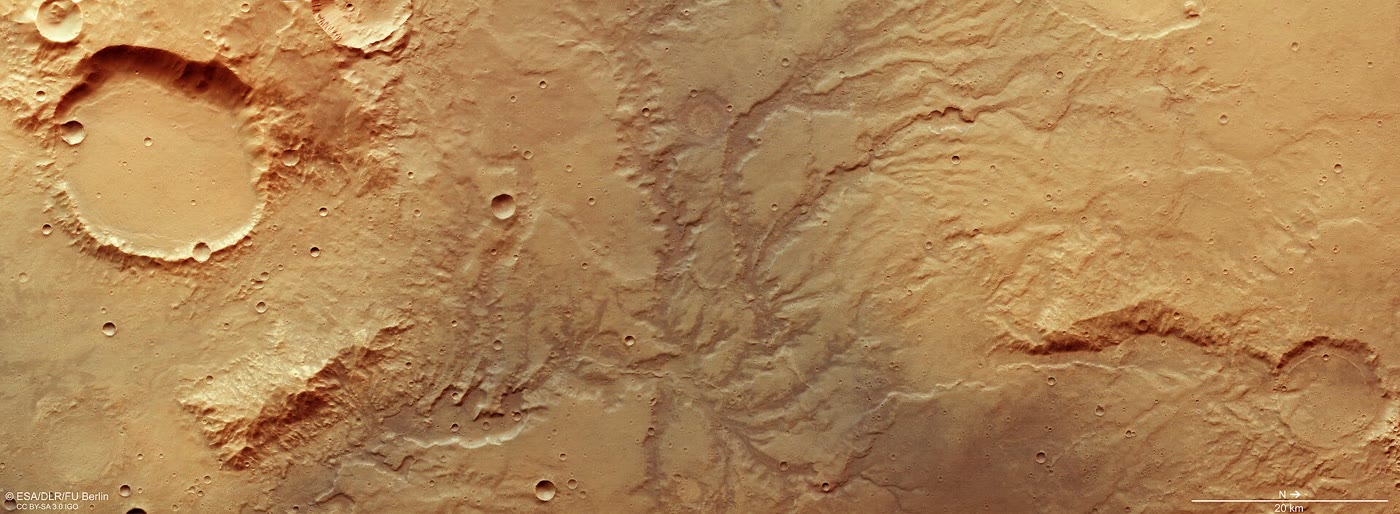
\includegraphics[width=\linewidth]{images/book5/b3-mars-valley-network.jpg}
\par\smallskip{\small 火星上干涸河谷的网络，由火星快车的
照相机拍摄，分辨率约为每像素 \qty{14}{m}，位于 南纬 \ang{17}、
东经 \ang{66} 附近；北在右侧，线段比例尺为 \qty{20}{km}。
支流在下游汇入较大的河谷，呈现出
流域水系的格局。图像：ESA/DLR/FU Berlin, CC BY-SA 3.0 IGO。}\label{fig:b3:planetary-atmospheres:valleys}
\end{omfigure}
% ledger: photo:b3-mars-valley-network

据地质估计，火星的河谷与水道需要
一层全球性的水，深 100 至 \qty{1500}{m}，而今日的火星冰与大气中仅
相当于 3 至 \qty{25}{m} 深的水层。其余大部分已逃逸到太空。
MAVEN 轨道器测得，太阳风剥离火星气体的速率约为
\qty{100}{g} 每秒，其中四分之三经行星背后的尾部流走，
即太阳风流动的方向；其余四分之一则以羽流形式
逸散于极区上空。在
2015 年 3 月的太阳风暴期间，流失加快，
在年轻的太阳更为活跃时，很可能快得多。火星还在流失氢，约
\num{3e26} 个原子每秒（今日平均），若持续四十亿年，
其损失仅相当于一层深约 \qty{4}{m} 的全球性水层。
% ledger: gilli25:h-loss, lasp:maven

这一速率并非始终与今日相同。火星的自转轴倾角如今为 \ang{25.2}，
过去 2.5 亿年间在 0 至 \ang{66} 之间变动，
围绕约 \ang{35} 的平均值摆动，而地球的倾角变化仅略多于
一度。这种运动是混沌的，无法回溯数十亿
年；擦边撞击形成的椭圆形撞击坑，其走向记录了倾角，
据此推断，过去约 35 亿年间平均倾角介于约 10 与 \ang{30} 之间。
倾角较大时，夏季极区升温，水汽上升更多，
气候模式计算出氢的流失速率可快二十倍：
在火星演化史上，流失量约相当于一层
深约 \qty{80}{m} 的水层。
% ledger: planet:Mars.obliq, gilli25:obliquity, holo18:obliquity, gilli25:h-loss

\section{土卫六：甲烷循环}\label{sec:b3:planetary-atmospheres:titan}

土卫六是一颗比火星还小的卫星，其大气比地球的更厚：
地表气压比地球高约 60\,\%，地表温度为 \qty{-179}{\degreeCelsius}。
大气约 95\,\% 为氮气、5\,\% 为甲烷，由于
该卫星引力较弱，其大气延伸高度为地球的十倍，
高度接近 \qty{600}{km}。紫外线在高空分解甲烷与氮气，
碎片重新结合，形成由较重碳氢化合物构成的橙色霾，
遮住地表，使可见光无法穿透。霾层之下，
甲烷起着水的作用：它凝结成云、降雨、
冲刷出河道，并充满甲烷与乙烷形成的湖泊和海。
% ledger: nasa:titan-surface, nasa:titan-facts

\begin{omfigure}
\centering
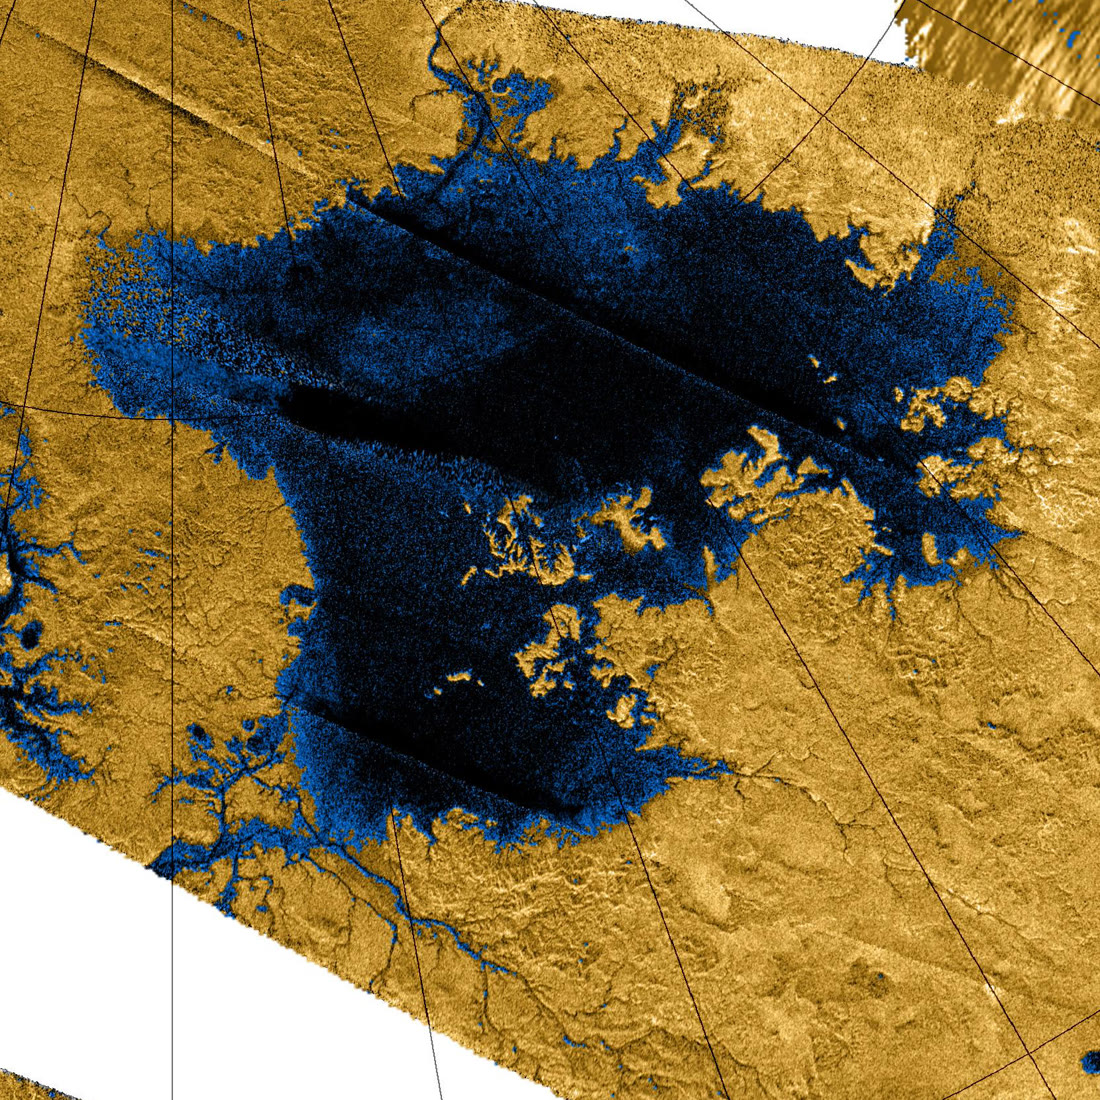
\includegraphics[width=0.5\linewidth]{images/book5/b3-ligeia-mare.jpg}
\par\smallskip{\small 利吉亚海，位于土卫六北极附近，为
卡西尼雷达图像的伪彩色拼接图：推测为液体的部分呈蓝色和黑色，
固体陆地呈棕色，并可见海湾、岛屿
与推测的支\omterm{def:b3:hydrogeology:flow-net}{流网}络。在所测绘的北部地区约 400 个湖泊与海中，
面积大于 \qty{26000}{km^2} 者占总面积的 70\,\%。
NASA/JPL/USGS，公有领域。}\label{fig:b3:planetary-atmospheres:ligeia}
\end{omfigure}
% ledger: photo:b3-ligeia-mare

液体能否存在于地表，取决于其相图以及
当地的压强与温度。土卫六地表略高于甲烷的
三相点（\qty{90.67}{K}，\qty{0.117}{bar}），并低于
其临界点。液态甲烷是可能存在的，而甲烷占 5\,\% 时，
其分压（以 \qty{1.6}{bar} 计）离饱和不远。火星地表接近水的
三相点，地球的地表远在其液相区内，而
金星地表高于水的临界温度 \qty{647}{K}，
在此温度下液体完全无法存在。
% ledger: nist:methane-phase, iapws:triple-critical, nasa:titan-surface

\begin{omfigure}
\centering
\begin{tikzpicture}
\begin{axis}[width=0.8\linewidth, height=0.52\linewidth,
  xmin=60, xmax=800, ymin=1e-4, ymax=1000, ymode=log,
  xlabel={温度 (\unit{K})}, ylabel={压强 (\unit{bar})},
  tick label style={font=\scriptsize}, label style={font=\small}]
\addplot[thick, omDef] table[x=T, y=p_bar] {figdata/out/bachelor-3-habitability-water.dat};
\addplot[thick, omDef, dashed] table[x=T, y=p_bar] {figdata/out/bachelor-3-habitability-ice.dat};
\addplot[thick, orange!80!black] table[x=T, y=p_bar] {figdata/out/bachelor-3-habitability-methane.dat};
\addplot[only marks, mark=*, mark size=1.6pt, omDef] coordinates {(273.16,0.00611657) (647.096,220.64)};
\addplot[only marks, mark=*, mark size=1.6pt, orange!80!black] coordinates {(90.67,0.1169) (190.6,46.1)};
\addplot[only marks, mark=square*, mark size=2.2pt, black] table[x=T, y=p_bar] {figdata/out/bachelor-3-habitability-bodies.dat};
\node[font=\scriptsize, anchor=south] at (axis cs:737,110) {金星};
\node[font=\scriptsize, anchor=west] at (axis cs:300,1.0) {地球};
\node[font=\scriptsize, anchor=north] at (axis cs:214,0.0045) {火星};
\node[font=\scriptsize, anchor=south] at (axis cs:94,2.2) {土卫六};
\node[font=\scriptsize, omDef, anchor=west] at (axis cs:420,3) {水：液态在上，蒸气在下};
\node[font=\scriptsize, omDef, anchor=north west] at (axis cs:205,0.0012) {冰};
\node[font=\scriptsize, orange!80!black, anchor=west] at (axis cs:196,46) {甲烷};
\node[font=\scriptsize, omDef, anchor=south east] at (axis cs:640,230) {临界点};
\end{axis}
\end{tikzpicture}
\par\smallskip{\small 蒸气与凝结水之间的边界
（蓝色：液体–蒸气，自三相点至临界点；
虚线：冰–蒸气）以及液态甲烷与其蒸气之间的边界（橙色），
并标出金星、地球、火星和土卫六地表的平均状态
（方块标记）。若地表压强高于某液体的
曲线之上，则该液体可以停留在地表，
前提是温度介于其三相点与临界点之间。}\label{fig:b3:planetary-atmospheres:phases}
\end{omfigure}
% ledger: iapws:vapour-pressure, iapws4:sublimation, iapws:triple-critical, nist:methane-phase, nasa:venus-atm, planet:Earth.Tmean, planet:Earth.psurf, nasa:mars-atm, nasa:titan-surface

土卫六易于保留氮气：在其\omterm{def:b3:planetary-atmospheres:exobase}{外逸层底}，氮的 $\lambda = 41$，
而氢的 $\lambda$ 约为 1.5，几乎可以自由逸出，而
分子氢的逸出则由更低处的极限通量所决定，
经过\omterm{def:b3:planetary-atmospheres:hydrodynamic}{均质层顶}，与地球上的情形相同。由断裂甲烷生成的
较重化合物沉降至地表，在那里构成
广袤沙丘区的沙子。
% ledger: gronoff:jeans-table, gronoff:diffusion, nasa:titan-surface

\section{行星宜居性}\label{sec:b3:planetary-atmospheres:habitability}

中学课本中的宜居带，是指距恒星的一段距离范围，
在此范围内，类地行星能够在其表面保有液态水。
其边界即本章中遇到的各种限制。

\begin{definition}[行星宜居性]\label{def:b3:planetary-atmospheres:habitability}
称一颗行星的\emph{行星宜居性}\index{行星宜居性}
是指其在地质时间尺度上能够保持地表液态水的能力：
它接收的恒星通量须位于
宜居带的范围之内，其大气与水须能抵抗
逃逸，并由长期碳循环调节其气候。
\end{definition}

宜居带的内缘即\omterm{def:b3:planetary-atmospheres:runaway}{湿温室效应}或\omterm{def:b3:planetary-atmospheres:runaway}{失控温室效应}：
绕太阳运行的类地行星在
\qty{0.99}{au} 处转为湿温室状态，在 \qty{0.97}{au} 处进入失控状态。外缘则是
外缘是\emph{最大温室效应}：加入二氧化碳只能使行星升温，直到
新增气体散回的太阳光超过其温室效应所得的
增益；对太阳而言，这一情形出现在
\qty{1.70}{au} 处，二氧化碳分压约为 \qty{8}{bar}。这些
保守的边界，计算时未考虑云层。另有两个经验边界更宽：
金星似乎至少 10 亿年没有地表水，
当时它所接收的阳光为地球现今的 1.76 倍（\qty{0.75}{au}）；
火星在接收阳光为地球现今 0.32 倍时仍有流水，若其
河谷年龄为 38 亿年（\qty{1.77}{au}）。较冷的恒星周围，同样的界限出现在
较低的通量处，因其光线偏红，散射较少而
更多地被水和二氧化碳吸收。
% ledger: kopparapu13:runaway, kopparapu13:outer, kopparapu13:hz-fit

\begin{omfigure}
\centering
\begin{tikzpicture}
\begin{axis}[width=0.8\linewidth, height=0.5\linewidth,
  xmin=0, xmax=2.1, ymin=2600, ymax=7200, x dir=reverse,
  xlabel={接收的恒星通量 / 今日地球},
  ylabel={恒星温度 (\unit{K})},
  tick label style={font=\scriptsize}, label style={font=\small},
  legend style={font=\scriptsize, at={(0.5,-0.24)}, anchor=north, legend columns=2, draw=none}]
\addplot[name path=mg, thick, omDef] table[x=mg, y=Teff] {figdata/out/bachelor-3-habitability-hz.dat};
\addlegendentry{湿温室效应}
\addplot[name path=maxg, thick, red!70!black] table[x=maxg, y=Teff] {figdata/out/bachelor-3-habitability-hz.dat};
\addlegendentry{最大温室效应}
\addplot[thin, omDef, dashed] table[x=rg, y=Teff] {figdata/out/bachelor-3-habitability-hz.dat};
\addlegendentry{失控温室效应}
\addplot[thin, black!60, densely dotted] table[x=rv, y=Teff] {figdata/out/bachelor-3-habitability-hz.dat};
\addlegendentry{近期金星、早期火星}
\addplot[thin, black!60, densely dotted, forget plot] table[x=em, y=Teff] {figdata/out/bachelor-3-habitability-hz.dat};
\addplot[green!30, opacity=0.5, forget plot] fill between[of=mg and maxg];
\addplot[only marks, mark=*, mark size=2pt, black, forget plot] coordinates {(1.911,5780) (1.0,5780) (0.431,5780)};
\node[font=\scriptsize, anchor=south] at (axis cs:1.911,5800) {金星};
\node[font=\scriptsize, anchor=west, xshift=2pt] at (axis cs:1.0,5780) {地球};
\node[font=\scriptsize, anchor=east, xshift=-2pt] at (axis cs:0.431,5780) {火星};
\end{axis}
\end{tikzpicture}
\par\smallskip{\small 类地行星的宜居带，以其接收的恒星通量对其恒星温度作图（
阴影区：\omterm{def:b3:planetary-atmospheres:runaway}{湿温室效应}与最大温室效应之间）。点线：由近期金星与早期火星
导出的经验界限。拟合曲线取自
无云气候模型，
适用范围为 2600 至
\qty{7200}{K}。}\label{fig:b3:planetary-atmospheres:hz}
\end{omfigure}
% ledger: kopparapu13:hz-fit, nasa:venus, nasa:mars

距离并不足够。行星必须保有其大气：
体积小或温度高的行星，其\omterm{def:b3:planetary-atmospheres:jeans-escape}{逃逸参数}较低，
会失去氢，进而失去水；处于\omterm{def:b3:planetary-atmospheres:runaway}{湿温室效应}状态的行星，
则会从顶部开始变干。行星还必须
在恒星逐渐变亮的数十亿年间保持气候稳定：
在地球上，长期碳循环中的硅酸盐风化恒温器
在气候变暖时吸收二氧化碳，在气候变冷时使其积累。
金星没有板块构造，脱气产生的二氧化碳
无法重新回到岩石中，于是在大气中不断积累；
如今它所含的二氧化碳量，大致与地球锁存于碳酸盐岩中的相当。
磁场是否保护大气尚有争议：它能使高层大气免受太阳风的侵袭，
但也开辟了其他逃逸途径，例如离子在极区附近的外流；
而且，行星能否宜居，
不能仅凭其在宜居带中的位置判断。
% ledger: arney18:venus-loss, gronoff21:magnetic, gronoff:nonthermal

\section{练习}

\begin{exercise}[$\star$]\label{exo:b3:planetary-atmospheres:1}
求金星表面附近的标高 $H = RT/Mg$，
所用数据依次为：金星（\qty{737}{K}，二氧化碳摩尔质量 \qty{44.01}{g.mol^{-1}}，
$g = \qty{8.87}{m.s^{-2}}$），地球（\qty{288}{K}，
\qty{28.97}{g.mol^{-1}}，\qty{9.80}{m.s^{-2}}），火星（\qty{214}{K}，
\qty{43.34}{g.mol^{-1}}，\qty{3.71}{m.s^{-2}}）和土卫六（\qty{94}{K}，
\qty{28.0}{g.mol^{-1}}，\qty{1.35}{m.s^{-2}}）的标高。哪种大气最为延展？
为什么？
\end{exercise}

\begin{exercise}[$\star$]\label{exo:b3:planetary-atmospheres:2}
地球的\omterm{def:b3:planetary-atmospheres:exobase}{外逸层底}位于 \qty{500}{km} 处（半径 \qty{6878}{km}）；其温度在太阳活动周期中
从 800 变化至 \qty{1600}{K}。取地球质量为 \qty{5.97e24}{kg}。
计算两种温度下氢原子的\omterm{def:b3:planetary-atmospheres:jeans-escape}{逃逸参数}，
以及逃逸比例 $(1 + \lambda)e^{-\lambda}$。
太阳活动周期使其改变了多少倍？
\end{exercise}

\begin{exercise}[$\star$]\label{exo:b3:planetary-atmospheres:3}
在太阳周围，一颗类地行星在通量 $S_\mathrm{eff}
= 1.014$ 处进入\omterm{def:b3:planetary-atmospheres:runaway}{湿温室效应}状态，在 1.0512 处失控，并在 0.3438 处达到最大温室效应状态。
（通量均以地球为基准）。(a)~计算这三个距离，
以天文单位表示。(b)~金星与火星所接收的阳光分别为地球的 1.91 倍和 0.43 倍，
将它们标出位置。
\end{exercise}

\begin{exercise}[$\star$]\label{exo:b3:planetary-atmospheres:4}
液态甲烷的水汽压为 $\log_{10}(p/\unit{bar}) = 3.9895 -
443.028/(T/\unit{K} - 0.49)$。(a)~计算其在土卫六表面
（\qty{94.15}{K}）时的值。(b)~甲烷占土卫六 \qty{1.6}{bar} 大气的 5\,\%，
计算其分压及相对湿度。(c)~
这一结果对土卫六海洋的蒸发说明了什么？
\end{exercise}

\begin{exercise}[$\star\star$]\label{exo:b3:planetary-atmospheres:5}
在地球的\omterm{def:b3:planetary-atmospheres:exobase}{外逸层底}（\qty{1000}{K}，氢的 $\lambda = 7.02$）处，计算氘的\omterm{def:b3:planetary-atmospheres:jeans-escape}{逃逸参数}、
其热运动速率相对于氢的比值，以及每个原子的金斯通量之比（氘对氢）。
\omterm{def:b3:planetary-atmospheres:jeans-escape}{金斯逃逸}是否为强的
同位素过滤器？
\end{exercise}

\begin{exercise}[$\star\star$]\label{exo:b3:planetary-atmospheres:6}
金星水的 D/H 比为 \num{0.016}，地球海水的
D/H 比为 \num{1.5575e-4}。(a)~计算富集倍数。(b)~若氘完全不逃逸，
则已知今日金星水量为 \qty{6e15}{kg}，其过去水量的最小值为多少？
若将其均匀铺展于该行星 \qty{4.60e14}{m^2} 的表面，水深为多少？(c)~若\omterm{def:b3:planetary-atmospheres:hydrodynamic}{扩散限制逃逸}
（$\alpha = 0.8$）要求储库缩小多少？
作出结论。
\end{exercise}

\begin{exercise}[$\star\star$]\label{exo:b3:planetary-atmospheres:7}
火星半径为 \qty{3389.5}{km}，每秒约失去 \num{3e26} 个氢原子。
(a)~若每两个原子来自一个水分子，则在四十亿年间，这一损失所移去的
全球水层厚度为多少？
(b)~若每秒失去 \num{6e27} 个原子（即高轴倾角时的速率），问题相同，结果如何？
(c)~将其与河谷和河道所需的 100 至 \qty{1500}{m}
相比较。
\end{exercise}

\begin{exercise}[$\star\star$]\label{exo:b3:planetary-atmospheres:8}
(a)~由火星的平均表面
压强 \qty{636}{Pa}、重力加速度 \qty{3.71}{m.s^{-2}} 和半径，计算火星大气的质量。
半径。(b)~太阳风每秒约剥去 \qty{100}{g} 气体。
这些损失在四十亿年间移去的质量为多少，
以及按此速率移去现今大气需要多长时间？(c)~为何这一结果低估了
过去的损失？
\end{exercise}

\begin{exercise}[$\star\star$]\label{exo:b3:planetary-atmospheres:9}
一颗具有无云水汽大气的类地行星，反射其接收太阳光的 19.3\,\%，
其红外输出不能超过
\qty{291}{W.m^{-2}}。(a)~太阳光通量（以每平方米瓦特计，相对地球的
\qty{1361}{W.m^{-2}}）超过多少时，该行星会失控？
(b)~将其与现今金星的 \qty{2601}{W.m^{-2}} 相比较，并与
太阳光度为现今 70\,\% 时的年轻金星相比较。(c)~为何
对年轻金星的结论并非最终的？
\end{exercise}

\begin{exercise}[$\star\star\star$]\label{exo:b3:planetary-atmospheres:10}
原子氧的模式热层为等温层，温度为 \qty{1000}{K}，其中
在 \qty{200}{km} 处 $n = \qty{1e16}{m^{-3}}$；取该高度处的 $g =
\qty{9.21}{m.s^{-2}}$，碰撞截面为
$\sigma_c = \qty{3e-19}{m^2}$。(a)~计算氧的标高。
(b)~计算\omterm{def:b3:planetary-atmospheres:exobase}{外逸层底}处的密度及\omterm{def:b3:planetary-atmospheres:exobase}{外逸层底}的高度。
(c)~重力随高度减小。这是否使\omterm{def:b3:planetary-atmospheres:exobase}{外逸层底}上移或
下移？
\end{exercise}

\begin{exercise}[$\star\star\star$]\label{exo:b3:planetary-atmospheres:11}
(a)~设地球平流层变为湿润，水汽混合比为
\num{3e-3}（以 $\ce{H2}$ 计）。扩散限制为
$\num{3.0e13}\,f$ 个 $\ce{H2}$ 分子（每平方厘米
每秒），温度为 \qty{200}{K}，计算整个
地球（半径 \qty{6371}{km}）的氢损失量。(b)~一个海洋（
\qty{1.4e24}{g} 水）可维持多久？与地球年龄相比较。
\end{exercise}

\begin{exercise}[$\star\star\star$]\label{exo:b3:planetary-atmospheres:12}
在以灰气体方式吸收的纯水汽高层大气中，其 $\kappa =
\qty{0.005}{m^2.kg^{-1}}$，行星上 $g = \qty{9.81}{m.s^{-2}}$
且 $D = 1.66$：(a)~计算辐射层的压强 $p_1$；
(b)~利用 $p_\mathrm{sat}(T) = \qty{611.657}{Pa}\,\exp[(L/R_v)(1/T_t -
1/T)]$, $L = \qty{2.5e6}{J.kg^{-1}}$, $R_v = \qty{461.5}{J.kg^{-1}.K^{-1}}$,
$T_t = \qty{273.16}{K}$，计算其温度及辐射极限。
(c)~逐线计算的极限为 \qty{291}{W.m^{-2}}。真实水汽的有效
$\kappa$ 应更大还是更小？
\end{exercise}

\section{问题：凯波斯能否保住它的水？}

\begin{problem}[{周末问题——虚构海洋行星的逃逸与
宜居性}]
\label{pb:b3:planetary-atmospheres:1}
凯波斯是一颗虚构的行星，质量为 \qty{5.2e24}{kg}，半径为
\qty{6200}{km}，具有海洋，大气由氮气和二氧化碳
组成。它以 \qty{0.60}{au} 的距离绕一颗恒星运行，其光度为太阳的 0.30 倍，
有效温度为 \qty{4800}{K}。其\omterm{def:b3:planetary-atmospheres:exobase}{外逸层底}位于
地表以上 \qty{500}{km}，温度为 \qty{1400}{K}，并含有
\qty{2e11}{m^{-3}} 个氢原子；其\omterm{def:b3:planetary-atmospheres:hydrodynamic}{均质层顶}温度为 \qty{200}{K}，
此处二氧化碳占主导，且氢的各种形式共同构成
混合比 $f = \num{1e-3}$（以 $\ce{H2}$ 计）。一个地球海洋的
\qty{1.4e24}{g} 水。

\medskip\noindent\textbf{第一部分——\omterm{def:b3:planetary-atmospheres:exobase}{外逸层底}。}
\begin{enumerate}
\item 计算凯波斯的表面重力加速度和平均密度。
\item 计算\omterm{def:b3:planetary-atmospheres:exobase}{外逸层底}处的逃逸速度。
\item 计算氢、氦和氧原子的热速率 $u = \sqrt{2kT/m}$，
  均取\omterm{def:b3:planetary-atmospheres:exobase}{外逸层底}处的值。
\item 计算它们的\omterm{def:b3:planetary-atmospheres:jeans-escape}{逃逸参数}。
\item 其中哪些可以以显著速率发生\omterm{def:b3:planetary-atmospheres:jeans-escape}{金斯逃逸}？
  是否有某一种接近\omterm{def:b3:planetary-atmospheres:hydrodynamic}{流体动力学逃逸}的情形？
\item 在其恒星活跃的早期，凯波斯的\omterm{def:b3:planetary-atmospheres:exobase}{外逸层底}温度可能曾达到
  \qty{3000}{K}。此时氢的\omterm{def:b3:planetary-atmospheres:jeans-escape}{逃逸参数}为多少，
  这说明了什么？
\end{enumerate}

\medskip\noindent\textbf{第二部分——氢的\omterm{def:b3:planetary-atmospheres:jeans-escape}{金斯逃逸}。}
\begin{enumerate}[resume]
\item 计算氢的 $(1 + \lambda)e^{-\lambda}$ 所表示的
  逃逸比例。
\item 计算氢的金斯通量，单位为每平方米每秒。
\item 计算每秒从整个\omterm{def:b3:planetary-atmospheres:exobase}{外逸层底}离开的
  氢原子数。
\item 一个地球海洋含有多少个氢原子？
\item 按此速率，凯波斯失去这些氢原子需要多长时间？
\item 计算氘的\omterm{def:b3:planetary-atmospheres:jeans-escape}{逃逸参数}，及其
  相对于氢、按每个原子计的逃逸效率。
\end{enumerate}

\medskip\noindent\textbf{第三部分——扩散限制。}
\begin{enumerate}[resume]
\item 计算\omterm{def:b3:planetary-atmospheres:hydrodynamic}{均质层顶}处二氧化碳的标高。
\item 氢在二氧化碳中的二元扩散参数为
  $b = \qty{1.2e19}{cm^{-1}.s^{-1}}$，温度为 \qty{200}{K}。计算
  $\ce{H2}$ 的扩散限制通量（每平方米每秒）。
\item 将其与地球极限 $\num{3.0e13}\,f$ 个分子每
  平方厘米每秒相比较，并按重力作换算。
\item 计算扩散限制每秒能为整个行星的高层大气
  提供的氢原子数（每秒），
  取行星的表面积计算。
\item 与问题~9 相比较。哪一过程限制了逃逸，
  以及热层中的氢将发生什么？
\item \omterm{def:b3:planetary-atmospheres:exobase}{外逸层底}处氢的密度须为多大，才能使\omterm{def:b3:planetary-atmospheres:jeans-escape}{金斯逃逸}
  带走全部供应量？
\item 凯波斯以扩散限制速率失去一个地球海洋
  所含的氢需要多长时间？
\end{enumerate}

\medskip\noindent\textbf{第四部分——凯波斯是否位于宜居带内？}
\begin{enumerate}[resume]
\item 计算凯波斯接收到的恒星通量，相对于地球的值。
\item 对于有效温度为 \qty{4800}{K} 的恒星，湿温室极限位于
  $S_\mathrm{eff} = 0.939$，最大温室极限位于 0.290。计算
  宜居带的内外边界（以天文单位计），并确定凯波斯的位置。
\item 恒星需增亮多少倍，凯波斯才会到达
  宜居带的内边界？
\item 取反照率为 0.3，计算凯波斯每平方米吸收的太阳光，
  及其平衡温度。与\omterm{def:b3:planetary-atmospheres:runaway}{失控
  温室极限}相比较。
\item 若更暖的气候使凯波斯的平流层变得湿润，其
  $f = \num{3e-3}$，一个地球海洋可维持多久？
\item 给出凯波斯失去一个地球海洋的氢所需的时间，
  通过\omterm{def:b3:planetary-atmospheres:hydrodynamic}{扩散限制逃逸}（取 $f = \num{1e-3}$），以十亿年为单位，
  保留两位有效数字。
\end{enumerate}
\end{problem}
% ledger: zahnle19:diffusion, kopparapu13:hz-fit, kopparapu13:runaway, gronoff:jeans, const:G, const:kB, const:NA
